\documentclass[dtu]{dtuarticle}
\usepackage{parskip} % use enters instead of indents

\newcommand{\todo}[1]{\color{red}[TODO: #1]\color{black}}
\newcommand*\chem[1]{\ensuremath{\mathrm{#1}}}
\usepackage{amsmath}
\usepackage{bm} % bold ITALIC math (for vectors!)
\usepackage{siunitx}
\usepackage{subcaption}

\title{Machine Learning Project 1}
\subtitle{Data: Feature extraction, and visualization}
\author{Group 94}
\course{02452 Machine Learning}
\address{
	DTU Compute \\
	Fall 2025
}
\date{\today}


\begin{document}

	\maketitle

	%	\begin{table}[h!]
		%		\renewcommand{\arraystretch}{1.1} % make the spacing a bit nicer
		%		\centering
		%		\begin{tabular}{l | l}
			%			\textbf{Name}                 & \textbf{Student number} \\ \hline\hline
			%			Vincent Van Schependom        & s251739                 \\ \hline
			%			Diego Armando Mijares Ledezma & s251777                 \\ \hline
			%			Albert Joe Jensen             & s204601
			%		\end{tabular}
		%		\caption{Group members.}
		%		\label{table:members}
		%	\end{table}
	%
	%	\begin{table}[h!]
		%		\renewcommand{\arraystretch}{1.1} % make the spacing a bit nicer
		%		\centering
		%		\begin{tabular}{l | *{3}{|l}}
			%			\textbf{Task} & \textbf{Vincent} & \textbf{Diego} & \textbf{Albert} \\ \hline\hline
			%			Section 1     & 30\%             & 30\%           & 40\%            \\ \hline
			%			Section 2     & 40\%             & 30\%           & 30\%            \\ \hline
			%			Section 3     & 30\%             & 40\%           & 30\%            \\ \hline
			%			Section 4     & 30\%             & 30\%           & 40\%			\\ \hline
			%			\LaTeX        & 90\%             & 5\%           & 5\%
			%		\end{tabular}
		%		\caption{Contributions \& responsabilities table.}
		%		\label{table:contributions}
		%	\end{table}

	\begin{table}[h!]
		\begin{subtable}{.58\textwidth}
			\begin{tabular}{l | l}
				\textbf{Name}                 & \textbf{Student number} \\ \hline\hline
				Vincent Van Schependom        & s251739                 \\ \hline
				Diego Armando Mijares Ledezma & s251777                 \\ \hline
				Albert Joe Jensen             & s204601
			\end{tabular}
			\caption{Group members.}
			\label{table:members}
		\end{subtable}
		\begin{subtable}{.4\textwidth}
			\begin{tabular}{l | *{3}{|l}}
				\textbf{Task} & \textbf{Vincent} & \textbf{Diego} & \textbf{Albert} \\ \hline\hline
				Section 1     & 30\%             & 30\%           & 40\%            \\ \hline
				Section 2     & 40\%             & 30\%           & 30\%            \\ \hline
				Section 3     & 30\%             & 40\%           & 30\%            \\ \hline
				Section 4     & 80\%             & 10\%           & 10\%			\\ \hline
				\LaTeX        & 90\%             & 5\%           & 5\%
			\end{tabular}
			\caption{Contributions \& responsabilities table.}
			\label{table:contributions}
		\end{subtable}
		\caption{Group information \& work distribution.}
	\end{table}

	\section*{Introduction}

	The objective of this report is to apply the methods that were discussed during the first
	section of the course \textit{Machine Learning} \cite{book} to a chosen dataset. The aim is to get
	a basic understanding of the data prior to the further analysis (project report 2).

	The particular dataset that is being investigated is the \textit{Glass Identification} dataset from 1987 by B. German \cite{dataset}. Table \ref{table:members} lists our full names and student numbers, while Table \ref{table:contributions} shows an overview of the contribution of each team member.

	\tableofcontents

	\newpage

	\section{The \textit{Glass Identification} dataset}

	The Glass Identification dataset \cite{dataset} comes from forensic science research in the 1980s, originally compiled at the Institute of Forensic Medicine, with support from the UCI Machine Learning Repository. It was created to help develop methods for identifying types of glass found at crime scenes, such as window glass, containers, or headlamps, based on their chemical makeup. The dataset has been widely shared since its inclusion in the UCI Repository in 1987, and it remains a popular benchmark for testing classification methods in research and teaching.

	\subsection{Previous analysis of the data}

	Several studies have analysed the dataset to improve multi-class classification performance. Zhou et al. applied machine learning techniques in 2023, focusing on optimising Support Vector Machines (SVM) through grid search and Bayesian methods \cite{zhou}. Their optimised SVM model achieved a remarkably high accuracy of 99.25\%, outperforming baseline models such as logistic regression, and demonstrated strong predictive ability when only chemical composition was available.

	In contrast, Bhowmick and Saha concentrated on addressing class imbalance and noisy data, also in 2023 \cite{bhowmick}. They removed outliers using interquartile range filtering, applied ReliefF feature ranking, and balanced classes with SMOTE before training an inverse-distance-weighted k-nearest-neighbor (kNN) classifier. Their improved pipeline reached 78.9\% accuracy with an $F$-measure of 0.791, showing how preprocessing can boost kNN’s effectiveness on this imbalanced dataset.

	\subsection{Goal}

	\todo{Explain, in the context of your problem of interest, what you hope to accom-
		plish/learn from the data using these techniques?}

	\todo{Explain which attribute you wish to predict in the regression based on which
		other attributes?}

	\todo{Which class label will you predict based on which other attributes in the classi-
		fication task?}

	\(\rightarrow\) (\textbf{V:}) The target variable is the type of glass (\texttt{type}), divided into 7 distinct classes. \todo{Complete this and tell that this will be the classification objective blabla.}

	\todo{Describe \textbf{main machine learning aim}: One of these tasks is likely more relevant than the rest and will be denoted the main machine learning aim in the following.}

	\(\rightarrow\) (\textbf{V:}) Mention that it's pretty obvious (and previously mentioned) that the main objective is \textbf{classification}.

	\subsection{Data transformations}

	\todo{Explain if you need to transform individual attribues in order to carry out these
		tasks (e.g. centering, standardization, discretization, log transform, etc.) and
		how you plan to do this.}

	\(\rightarrow\) (\textbf{V:}) I would just mention overall standardisation is necessary, since it's all on different scales, a bit like in the PCA section (maybe move the text from there over here, and afterwards say something like ``As we already mentioned in Section ..., standardisation is necessary'' in the PCA section.). Also refer to the boxplots (unscaled and scaled).

	\section{A close look at the different attributes}

	``Assignment: \textit{Describe if the attributes are discrete/continuous and whether they are nominal/or-
		dinal/interval/ratio.}''

	The data set consists of 214 samples of glass, each characterised by glass type, along with 9 numeric features. There are \textit{no missing values}. The attributes are all presented in Table \ref{table:attributes} and the \texttt{type} attribute is unfolded in Table \ref{table:types}.

	The refractive index (\texttt{RI}), and concentrations of eight different oxides, including sodium (\texttt{Na}), magnesium (\texttt{Mg}), aluminum (\texttt{Al}), silicon (\texttt{Si}), potassium (\texttt{K}), calcium (\texttt{Ca}), barium (\texttt{Ba}), and iron (\texttt{Fe}) all are \textit{continuous} and \todo{ratio or interval}.

	\begin{table}
		\centering
		%\renewcommand{\arraystretch}{1.3} % make the spacing a bit nicer
		\begin{tabular}{l|l|l}
			\textbf{Attribute} & \textbf{Description}                    & \textbf{Type of variable} \\ \hline \hline
			\texttt{ID}        & Observation ID (excluded from analysis) & Numeric (discrete)        \\ \hline
			\texttt{RI}        & Refractive Index                        & Continuous                \\ \hline
			\texttt{Na}        & Sodium oxide ($\chem{Na_2 O}$)          & Continuous                \\ \hline
			\texttt{Mg}        & Magnesium oxide ($\chem{Mg O}$)         & Continuous                \\ \hline
			\texttt{Al}        & Aluminum oxide ($\chem{Al_2 O_3}$)      & Continuous                \\ \hline
			\texttt{Si}        & Silicon oxide ($\chem{Si O_2}$)         & Continuous                \\ \hline
			\texttt{K}         & Potassium oxide ($\chem{K_2 O}$)        & Continuous                \\ \hline
			\texttt{Ca}        & Calcium oxide ($\chem{Ca O }$)          & Continuous                \\ \hline
			\texttt{Ba}        & Barium oxide ($\chem{Ba O}$)            & Continuous                \\ \hline
			\texttt{Fe}        & Iron oxide ($\chem{Fe_2 O_3}$)          & Continuous                \\ \hline
			\texttt{type}      & Type of glass                           & Nominal                   \\
		\end{tabular}
		\caption{\todo{Fill in.}}
		\label{table:attributes}
	\end{table}

	\begin{table}
		\centering
		%\renewcommand{\arraystretch}{1.3} % make the spacing a bit nicer
		\begin{tabular}{r|l|l}
			\textbf{} & \textbf{Abbreviation in dataset} & \textbf{Description}                 \\ \hline\hline
			1 & \texttt{BW-FP}                   & Building Window, Float Processed     \\ \hline
			2 & \texttt{BW-NFP}                  & Building Window, Non Float Processed \\ \hline
			3 & \texttt{VW-FP}                   & Vehicle Window, Float Processed      \\ \hline
			4 & \texttt{VW-NFP}                  & Vehicle Window, Non Float Processed  \\ \hline
			5 & \texttt{containers}              & Containers                           \\ \hline
			6 & \texttt{tableware}               & Tableware (e.g. \dots)               \\ \hline
			7 & \texttt{headlamps}               & Headlamps (e.g. \dots)
		\end{tabular}
		\caption{\todo{Fill in.}}
		\label{table:types}
	\end{table}

	\section{Descriptive analysis of the dataset}

%	Based on the summary statistics in Table \ref{table:summary-stats}, several attributes in the Glass dataset exhibit high variance or distributional irregularities that could introduce noise. \texttt{Mg} and \texttt{Ca} both have relatively large standard deviations (1.44 and 1.42), indicating wide dispersion compared to other features. \texttt{K} is the most problematic, with a low mean (0.50) but a similarly large standard deviation (0.65), combined with extreme skewness (6.55) and very high kurtosis (54.69), suggesting the presence of rare but extreme outliers. \texttt{Ba} also shows notable skewness (3.42) and kurtosis (12.54), reflecting occasional extreme values against mostly near-zero observations. Fe displays moderate skew (1.75) and kurtosis (2.66), though its absolute values remain small.
%
%	These patterns suggest that robust handling, through transformations, scaling, or outlier mitigation, may be most important for \texttt{K}, \texttt{Ba}, and \texttt{Fe}, while \texttt{Mg} and \texttt{Ca} may benefit from normalisation.

	\subsection{Summary statistics}

	\todo{The assignment is as follows:}

	\textit{``Include relevant summary statistics of the attributes. Reflect on the values.
		If your data set contains many similar attributes, you may restrict yourself to describing a
		few representative features (apply common sense). You can place additional results in the
		appendix if needed.''}

	\todo{Reshuffle the text such that it follows the structure of this \LaTeX document.}

%	Based on the summary statistics in Table \ref{table:summary-stats} and the histograms in Figure \ref{fig:histograms}, several attributes in the Glass dataset display variance patterns or irregular distributions. \texttt{K} is the most problematic, with extreme skewness and heavy tails; its histogram shows many zeros and a few very large outliers, consistent with its high kurtosis.
%
%	Ba and \texttt{Fe} follow a similar pattern, with distributions dominated by near-zero values and occasional spikes, making them highly skewed and potentially noisy. \texttt{Mg} exhibits a bimodal distribution, with one cluster near zero and another around 3–4, suggesting that variation may partly reflect differences between glass types, though still requiring careful treatment.
%
%	\texttt{Ca} has high spread but a more balanced shape. By contrast, \texttt{RI}, \texttt{Na}, \texttt{Al}, and \texttt{Si} appear roughly symmetric. Transformations (log or Box-Cox), standardization, or winsorization are recommended for skewed features, while Mg’s multimodality may warrant class-sensitive preprocessing.

%	Attributes like \texttt{Na}, \texttt{Si}, and \texttt{Ba} have relatively symmetric boxes and whiskers in their boxplots in Figure \ref{fig:boxplots}, suggesting that they are closer to a normal distribution after standardization. In contrast, \texttt{RI}, \texttt{Mg}, \texttt{Al}, \texttt{K}, and \texttt{Ca} exhibit noticeable skewness and numerous outliers, indicating clear deviations from normality.

	\todo{Put boxplots, histograms.}

	\subsection{Extreme values and outliers}

	\todo{Reshuffle the text such that it follows the structure of this \LaTeX document.}

	\todo{Mention boxplots.}

	\begin{figure}
		\centering
		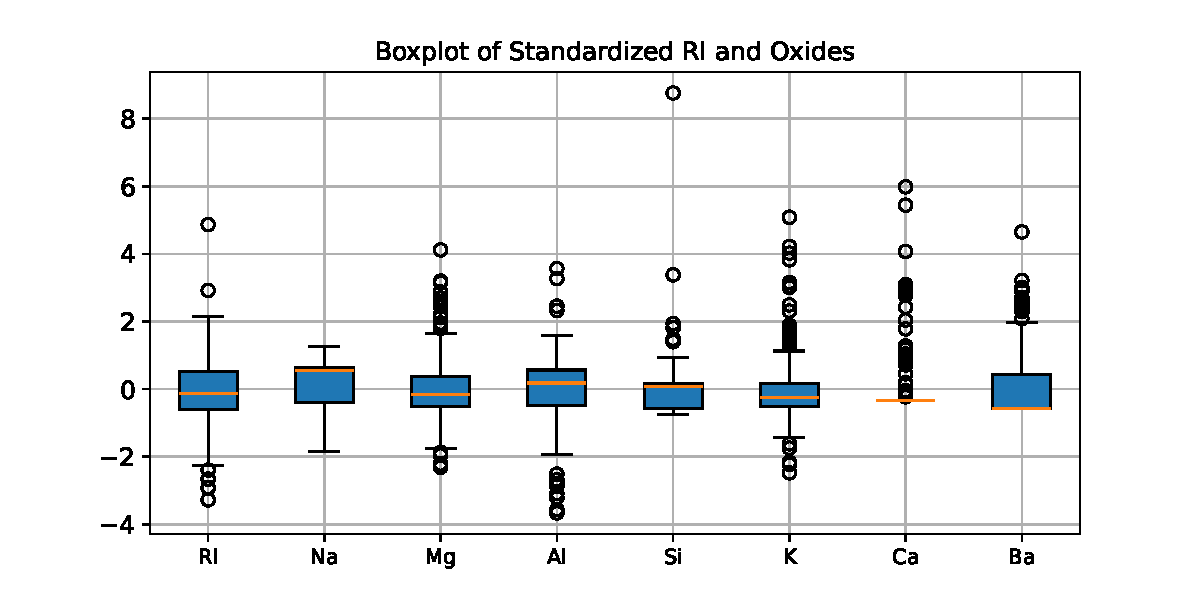
\includegraphics[width=.8\textwidth]{figures/boxplots}
		\caption{Boxplots of the refractive index (\texttt{RI}) and the 8 oxides.}
		\label{fig:boxplots}
	\end{figure}

	\subsection{Distribution of the attributes}

	\todo{Reshuffle the text such that it follows the structure of this \LaTeX document.}

	The distribution of the glass type - as can be see in Table \ref{table:frequencies} - is imbalanced: 70 float-processed building windows, 76 processed building windows, 17 vehicle windows, 13 containers, 9 tableware, and 29 headlamps. Class 4 (\texttt{VW-NFP}) has no samples

	\label{section:distribution}

	\begin{figure}
		\centering
		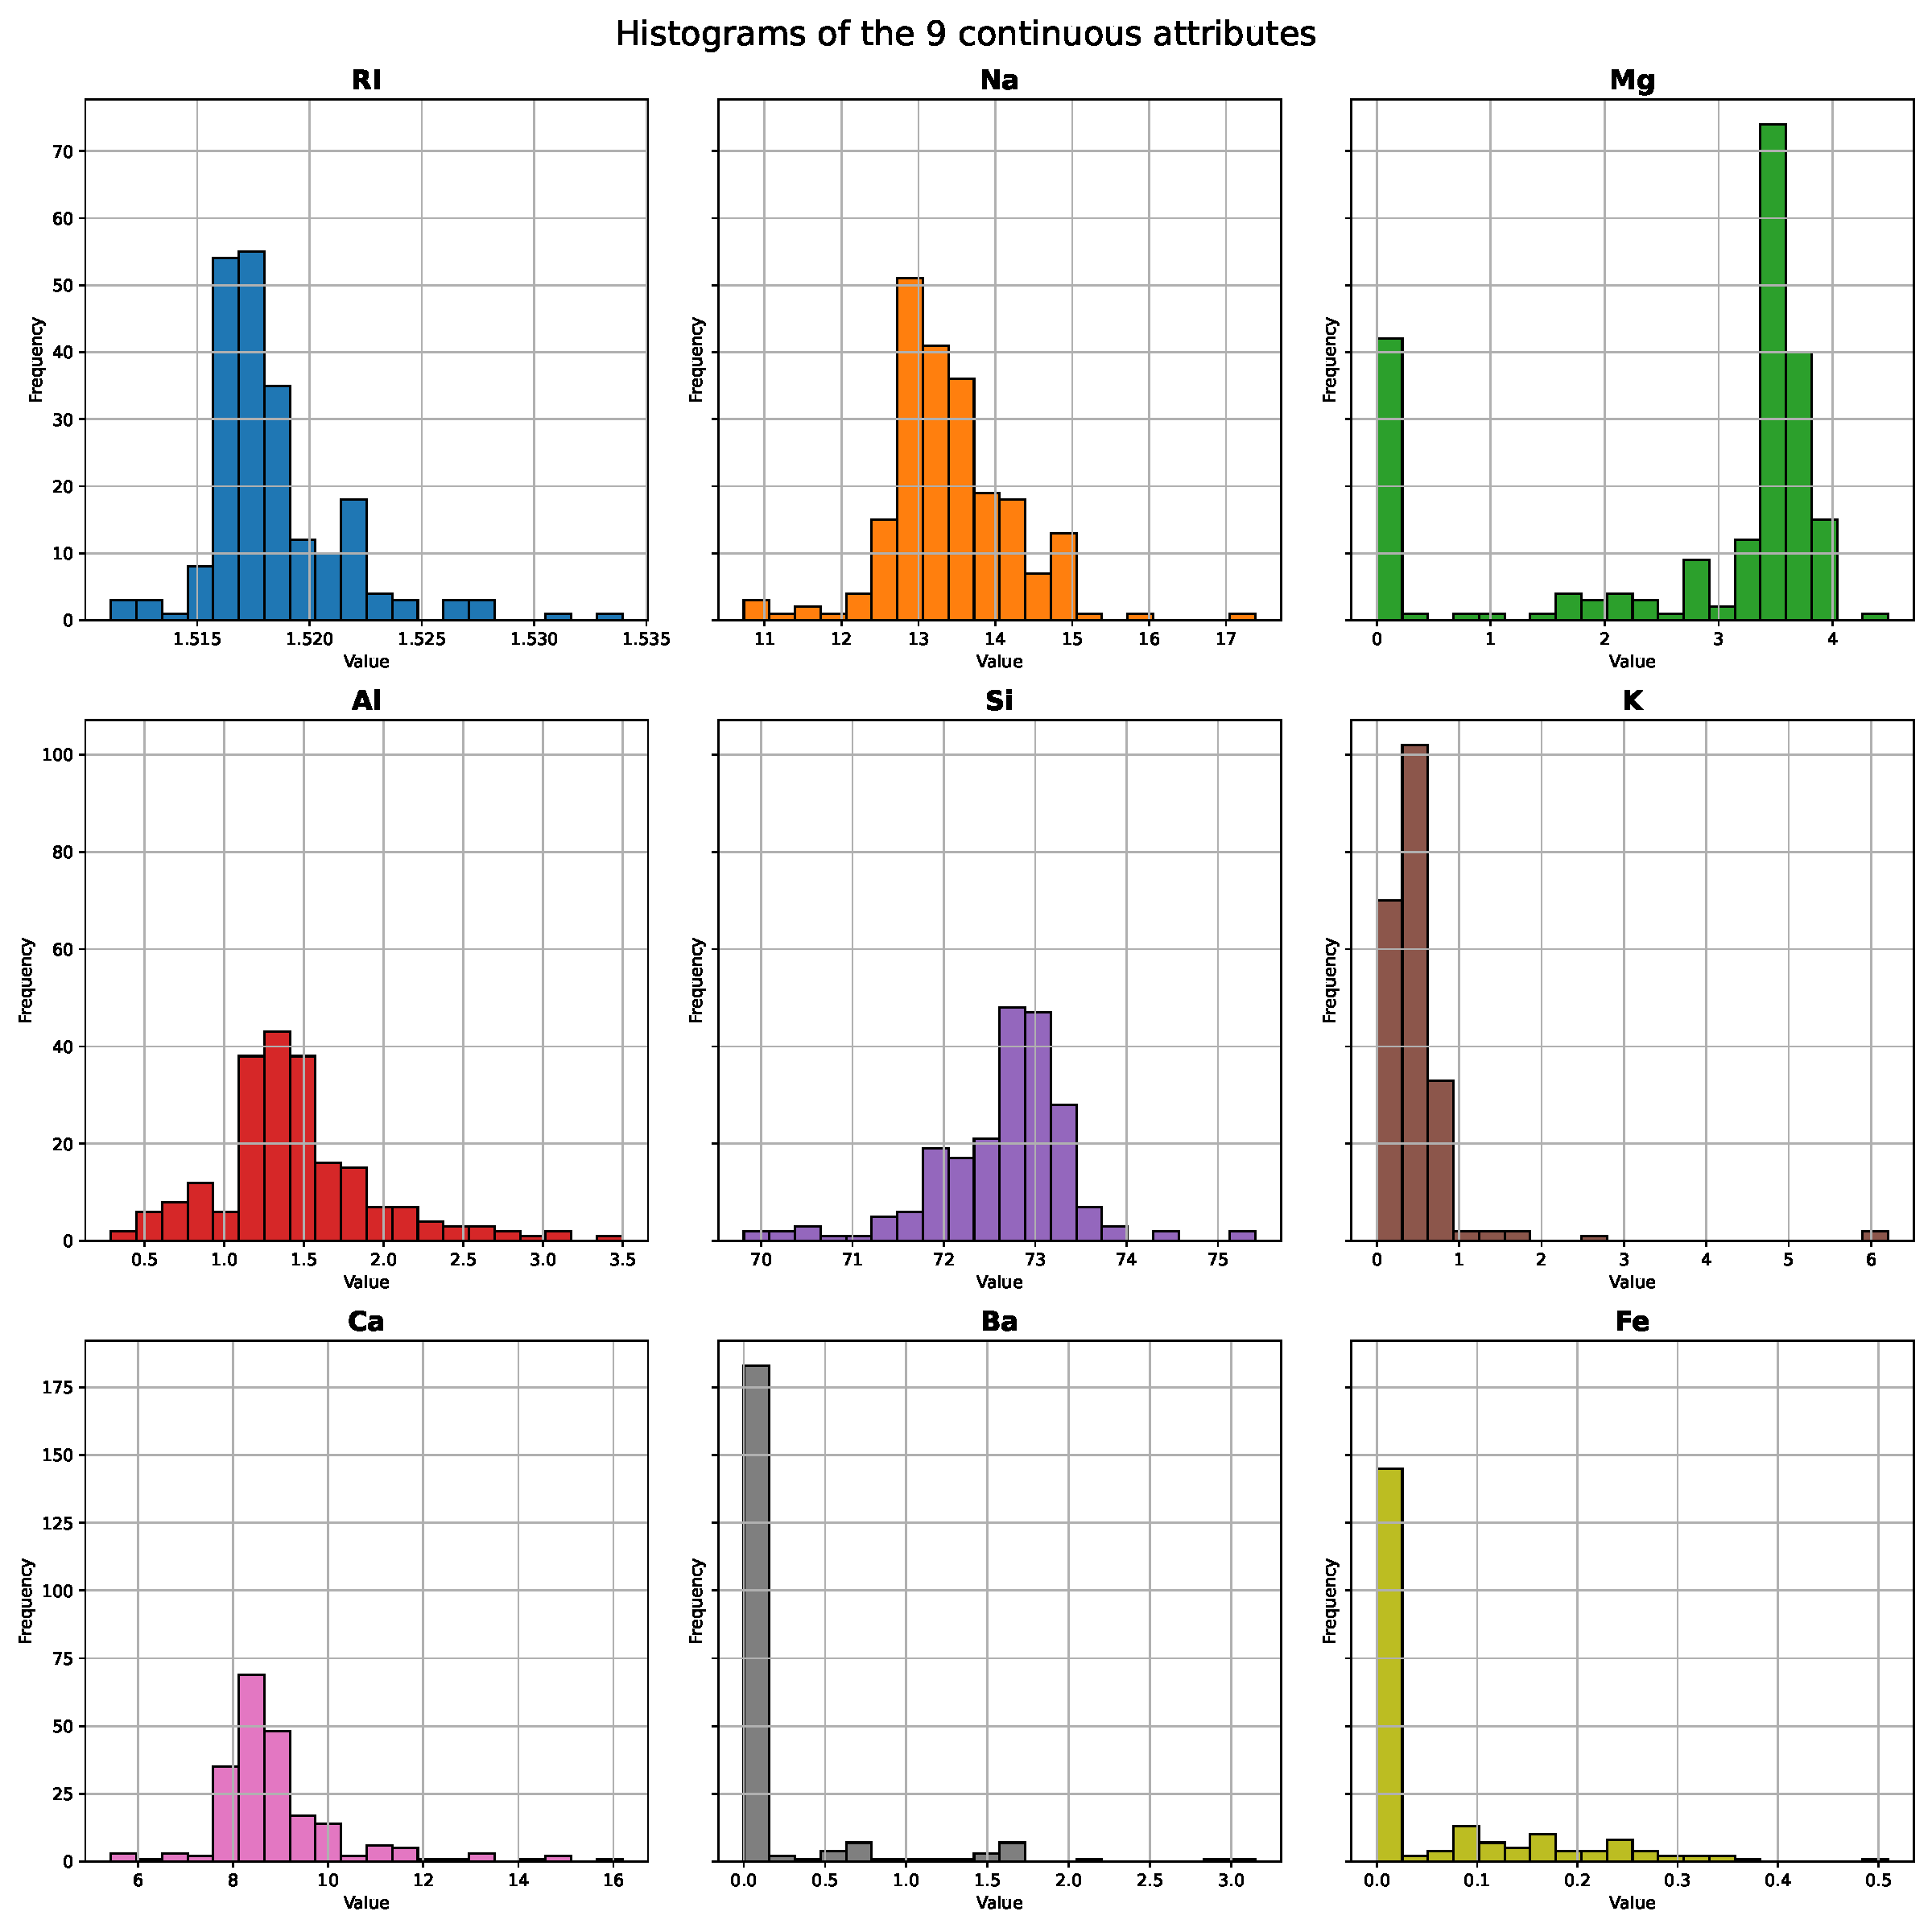
\includegraphics[width=.8\textwidth]{figures/histograms}
		\caption{Relative frequency histograms for the nine numerical attributes. \todo{Describe the general distributions.}}
		\label{fig:histograms}
	\end{figure}

	\todo{Mention the histograms and maybe the boxplots, too.} (Figure \verb*|\ref{fig:histograms}|)

	\begin{table}[h!]
		\centering
		\begin{subtable}{0.65\textwidth}
			\begin{tabular}{r | *{6}{| r}}
				& \textbf{Mean} & \textbf{Std.} & \textbf{Min} & \textbf{Max} & \textbf{Skew} & \textbf{Kurtosis} \\ \hline\hline
				\texttt{RI} & 1.518 & 0.003 & 1.511 & 1.534 & 1.625 & 4.932 \\ \hline
				\texttt{Na} & 13.408 & 0.817 & 10.730 & 17.380 & 0.454 & 3.052 \\ \hline
				\texttt{Mg} & 2.685 & 1.442 & 0.000 & 4.490 & -1.153 & -0.410 \\ \hline
				\texttt{Al} & 1.445 & 0.499 & 0.290 & 3.500 & 0.907 & 2.061 \\ \hline
				\texttt{Si} & 72.651 & 0.775 & 69.810 & 75.410 & -0.730 & 2.968 \\ \hline
				\texttt{K} & 0.497 & 0.652 & 0.000 & 6.210 & 6.552 & 54.690 \\ \hline
				\texttt{Ca} & 8.957 & 1.423 & 5.430 & 16.190 & 2.047 & 6.682 \\ \hline
				\texttt{Ba} & 0.175 & 0.497 & 0.000 & 3.150 & 3.416 & 12.541 \\ \hline
				\texttt{Fe} & 0.057 & 0.097 & 0.000 & 0.510 & 1.754 & 2.662
			\end{tabular}
			\caption{Summary statistics.}
			\label{table:summary-stats}
		\end{subtable}
		\hspace*{0.02\textwidth}
		\begin{subtable}{.3\textwidth}
			\begin{tabular}{r|l|r|r}
				& \texttt{type}       & \textbf{Cnt.} & \textbf{Freq.} \\ \hline\hline
				1 & \texttt{BW-FP}      & 70 & 0.327 \\ \hline
				2 & \texttt{BW-NFP}     & 76 & 0.355 \\ \hline
				3 & \texttt{VW-FP}      & 17 & 0.079 \\ \hline
				4 & \texttt{VW-NFP}     & 0  & 0.000 \\ \hline
				5 & \texttt{containers} & 13 & 0.061 \\ \hline
				6 & \texttt{tableware}  & 9  & 0.042 \\ \hline
				7 & \texttt{headlamps}  & 29 & 0.136
			\end{tabular}
			\caption{Absolute and relative frequencies of \texttt{type}.}
			\label{table:frequencies}
		\end{subtable}
		\caption{Summary statistics of continuous variables and frequency distribution of glass \texttt{type}.}
	\end{table}


	\subsection{Correlation between attributes}

	\todo{Fill out this section.}

	\begin{figure}[h!]
		\centering
		\begin{subfigure}{.49\textwidth}
			\centering
			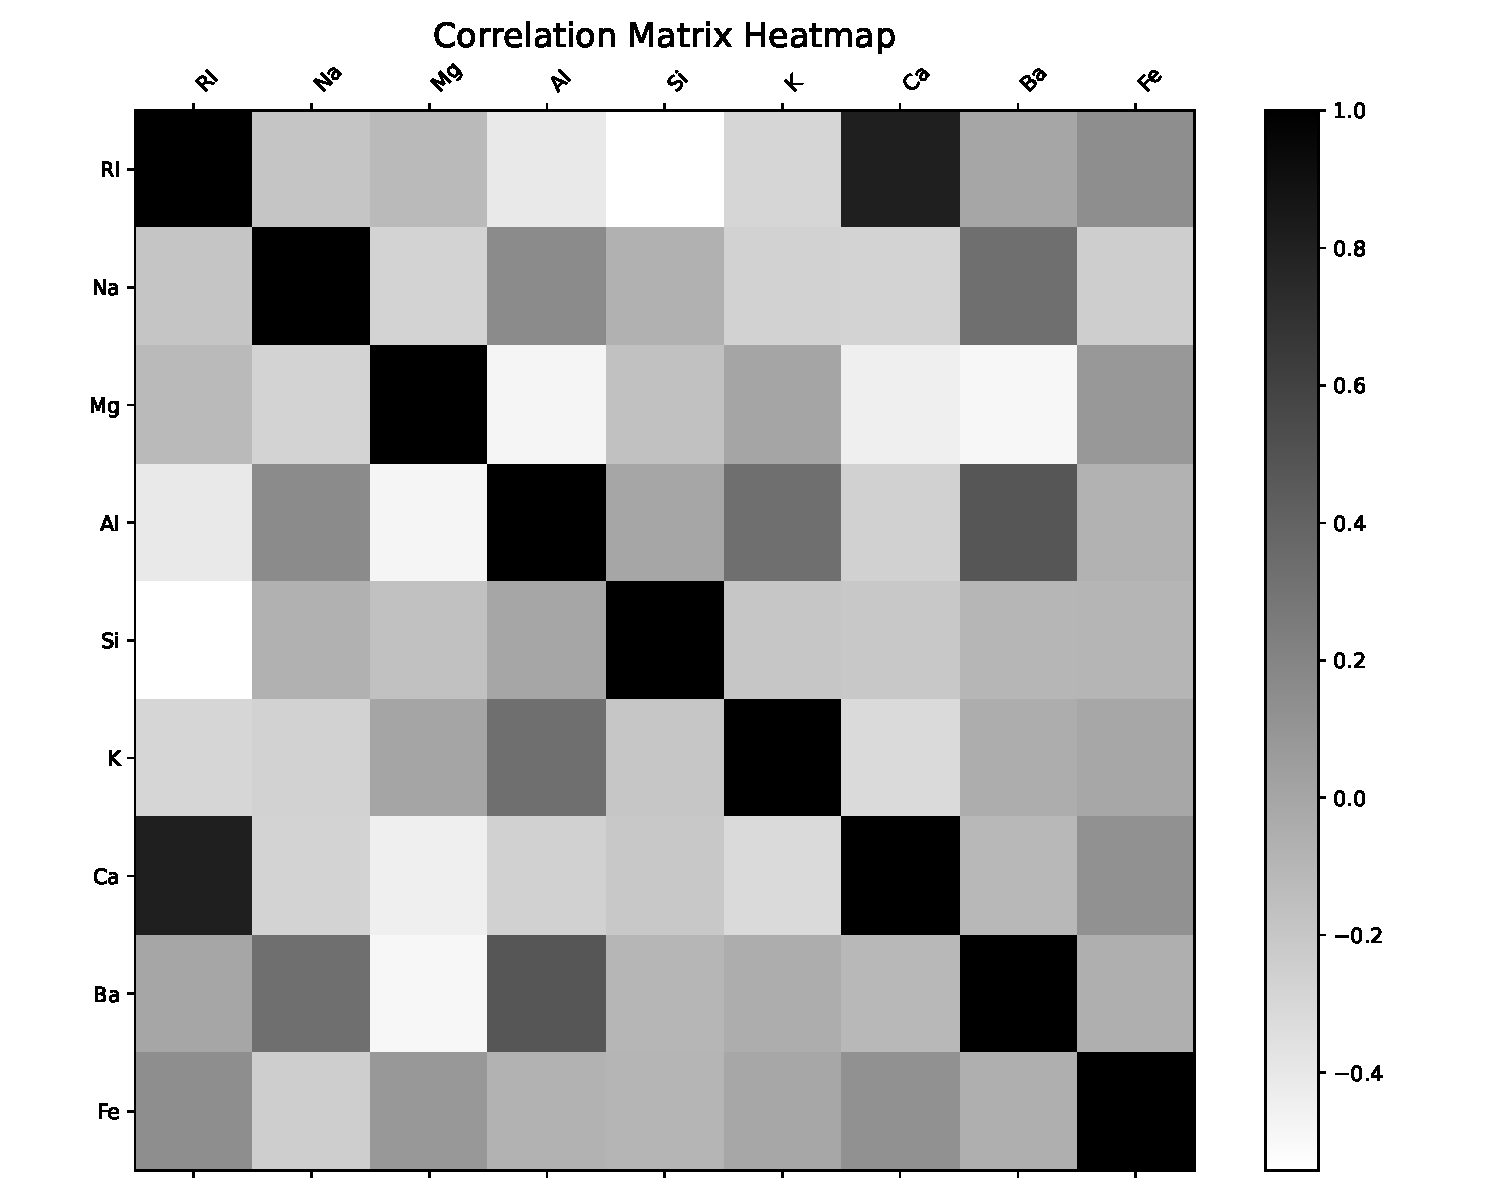
\includegraphics[width=\textwidth]{figures/correlation_matrix}
			\caption{Correlation matrix for the nine numerical attributes.}
			\label{fig:correlation}
		\end{subfigure}
		\begin{subfigure}{.49\textwidth}
			\centering
			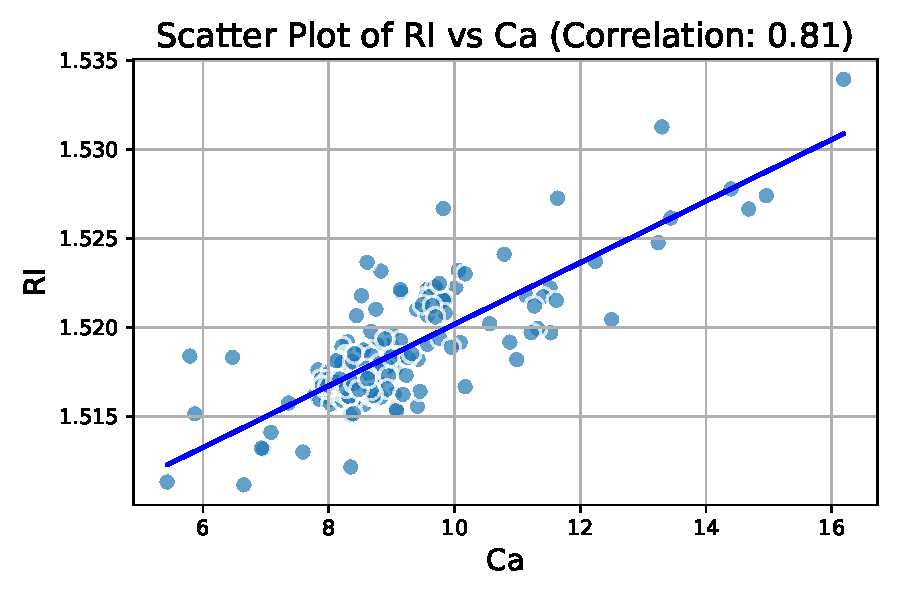
\includegraphics[width=\textwidth]{figures/scatter_RI_vs_Ca}
			\caption{Individual correlation between \texttt{RI} and \texttt{Ca}}
			\label{fig:individual-correlation}
		\end{subfigure}
		\caption{Whole correlation matrix and individual correlation between \texttt{RI} and \texttt{Ca}.}
	\end{figure}

	\todo{Reference the matrix correlation plot.}  (Figure \verb*|\ref{fig:correlation}|)

	\section{Principal Component Analysis}

	\subsection{Need for standardisation}

	Since the attributes are expressed on different numerical scales (see Section \ref{section:distribution}), the variables are standardised by subtracting the mean and dividing by the standard deviation. This ensures that no single attribute dominates the analysis merely due to its scale.

	\subsection{Dimension reduction}

	\begin{figure}[h!]
		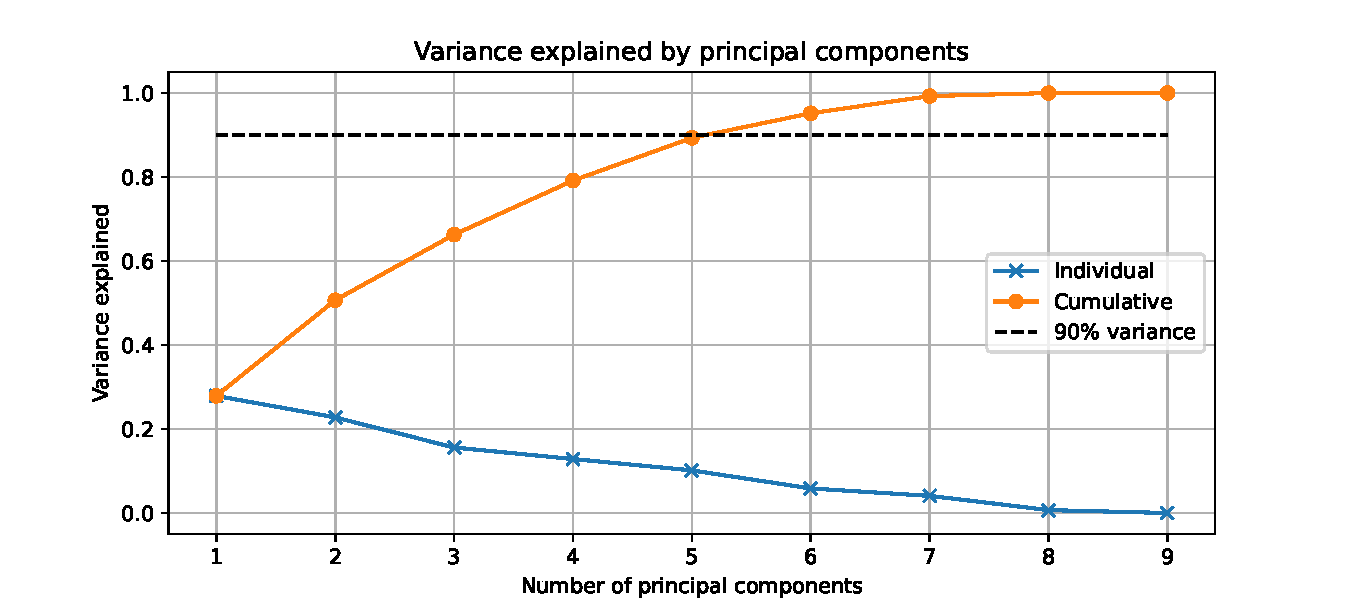
\includegraphics[width=.9\textwidth]{figures/pca_explained_variance}
		\caption{Explained (cumulative) variances for the 9 principal components $\bm{v}_0,\ldots,\bm{v}_8$}.
		\label{fig:explained-var}
	\end{figure}

	The goal is to reduce the original 9-dimensional dataset to an $M$-dimensional representation with $M < 9$, using the first $M$ principal components $\bm{v}_0,\ldots,\bm{v}_{M-1}$. As shown in Figure \ref{fig:explained-var}, selecting $M=5$ principal components explains \SI{89.31}{\percent} of the total variance. By increasing the dimensionality to $M=7$, as much as \SI{99.27}{\percent} of the variance can be retained, essentially preserving almost all of the original information.

	Choosing $M=5$ provides a balance between dimensionality reduction and information retention. While $M=7$ captures nearly all of the variance, the marginal gain in explained variance beyond the first five components is relatively small compared to the added complexity. Retaining five dimensions reduces computational cost, simplifies subsequent analysis, and removes noise while still preserving the majority of the data's variability.

	\subsection{Principal directions}

	The \textit{principal directions} of the first $M$ principal components are defined by the eigenvectors $\bm{v}_i$ that span the subspace of reduced dimensionality. These vectors form the transformation matrix $\bm{V}_M$, which is applied to the standardised data $\bm{X}$ to obtain the projected representation $\bm{B} = \bm{V}_M \bm{X}$. The new coordinates $\bm{B}$ capture the structure of the data in fewer dimensions while emphasising the directions of greatest variance.

	\begin{table}[h!]
		\centering
		\begin{tabular}{r | *{5}{|r}}
			\textbf{Variable} & $\textbf{PC}_0$ & $\textbf{PC}_1$ & $\textbf{PC}_2$ & $\textbf{PC}_3$ & $\textbf{PC}_4$ \\ \hline\hline
			\texttt{RI} & \num{0.545}     &          -0.286 &           0.087 &          -0.147 &          -0.074 \\
			\texttt{Na} & -0.258          &          -0.270 &          -0.385 &          -0.491 &           0.154 \\
			\texttt{Mg} & 0.111           &           0.594 &           0.008 &          -0.379 &           0.124 \\
			\texttt{Al} & -0.429          &          -0.295 &           0.329 &           0.138 &           0.014 \\
			\texttt{Si} & -0.229          &           0.155 &          -0.459 &           0.653 &           0.009 \\
			\texttt{K} & -0.219          &           0.154 &           0.663 &           0.039 &          -0.307 \\
			\texttt{Ca} & 0.492           &          -0.345 &          -0.001 &           0.276 &          -0.188 \\
			\texttt{Ba} & -0.250          &          -0.485 &           0.074 &          -0.133 &           0.251 \\
			\texttt{Fe} & 0.186           &           0.062 &           0.284 &           0.230 &           0.873
		\end{tabular}
		\caption{The principal directions (a.k.a. the \textit{loadings}) of the first $M=5$ principal components $\text{PC}_i = \bm{v}_i$ in the rotation matrix $\bm{V}_M$. Larger absolute values indicate stronger influence of a variable on a given component.}
		\label{table:loadings}
	\end{table}

	\begin{figure}
		\centering
		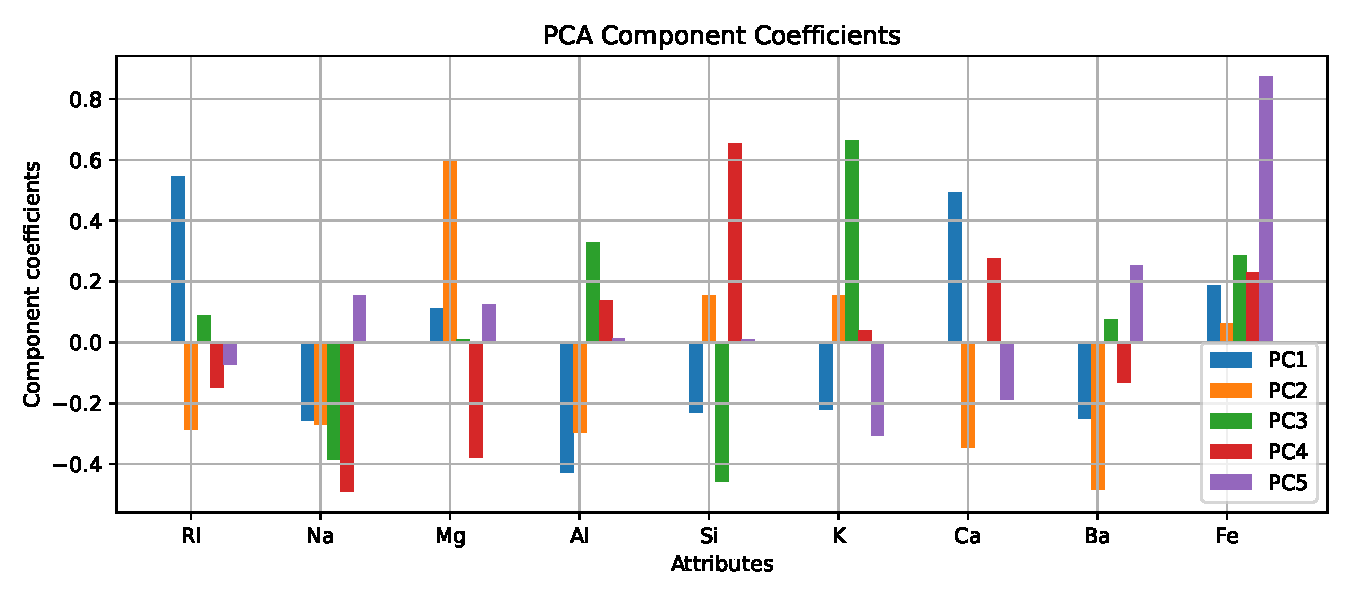
\includegraphics[width=.99\textwidth]{figures/pca_component_coefficients}
		\caption{Loadings of the original variables on the first five principal components. Positive and negativ values indicate the \textit{direction} of influence, while the magnitude reflects the \textit{strength} of the contribution.}
		\label{fig:pc-components}
	\end{figure}

	Based on the loadings in Table \ref{table:loadings} and the corresponding visualisation in Figure \ref{fig:pc-components}, the first principal component ($\text{PC}_0$) is most strongly influenced by \texttt{RI} and \texttt{Ca}, which carry positive loadings, and negatively by \texttt{Al} and \texttt{Si}. This suggests that $\text{PC}_0$ captures a trade-off between refractive index and calcium content versus aluminium and silicon.

	%	Shortened version of the stuff that is beneath this comment:
	%	The second principal component ($\text{PC}_1$) places strong weight on \texttt{Mg} and negative weight on \texttt{Ba}, indicating a contrast between magnesium and barium content. Later components highlight more specific variations, such as $\text{PC}_4$, which is dominated by \texttt{Fe}, pointing to a component that largely isolates variation in iron concentration.

	\todo{Review all the stuff that is below and check for errors.}

	The second principal component ($\text{PC}_1$) assigns a large positive loading to \texttt{Mg}, while strongly down-weighting \texttt{Ba} and, to a lesser degree, \texttt{Na}. This indicates that $\text{PC}_1$ primarily reflects a contrast between magnesium concentration and the presence of barium and sodium.

	The third principal component ($\text{PC}_2$) is dominated by a large positive loading for \texttt{K}, balanced by strong negative contributions from \texttt{Si} and \texttt{Na}. This points to a dimension that separates potassium-rich compositions from those with higher silica and sodium content.

	The fourth principal component ($\text{PC}_3$) shows high positive contributions from \texttt{Si}, \texttt{Ca}, and \texttt{Fe}, with negative influence from \texttt{Mg} and \texttt{Na}. It therefore captures variation where higher levels of silicon, calcium, and iron occur together in opposition to magnesium and sodium.

	Finally, the fifth principal component ($\text{PC}_4$) is characterised by a dominant positive loading for \texttt{Fe}, while moderately influenced by \texttt{Ba} and negatively by \texttt{K}. This indicates that $\text{PC}_4$ primarily isolates variation in iron concentration, with some contribution from the balance between barium and potassium.

	\subsection{Projected data}

	\subsubsection{Biplots}

	The projection of the standardised dataset onto the principal component axes produces a lower-dimensional representation that can be visualised in two-dimensional \textit{biplots}. In these plots:

	\begin{itemize}
		\item Each point corresponds to a \textit{score}, representing the coordinates of an original observation in the space spanned by the selected principal components. The scores have been \textit{rescaled} to the interval $[-1,1]$ to facilitate comparison with the arrows, representing variable loadings.
		\item The arrows correspond to the \textit{loadings}, i.e., the contributions of the original variables to the principal components. The direction of an arrow indicates how the variable influences the component axes, and its length reflects the magnitude of this influence.
	\end{itemize}

	Together, scores and loadings allow for simultaneous interpretation of both the observations and the variables.

	\subsubsection{Interpretation based on glass types}

	Figure~\ref{fig:biplots} shows two biplot visualisations. In the first biplot (PC1 vs.\ PC2), which captures \SI{50}{\percent} of the variance, the dominant trends in the data are visible, and some separation between glass types can be observed \todo{explain}. For the second biplot, \todo{fill out.}

	\todo{Check the paragraph below and fill out further.}

	The projected scores reveal that some classes, such as \texttt{BW-FP} and \texttt{R}, cluster distinctly in the reduced space, whereas others, such as \texttt{LW-FP} and \texttt{GL}, exhibit more overlap. The loadings indicate that the separation of classes along the axes is largely driven by specific chemical compositions; for example, PC1 contrasts samples with high \texttt{RI} and \texttt{Ca} against those with higher \texttt{Al} and \texttt{Si}, explaining why some classes separate along this component. \todo{Explain the concrete projections of the different classes further.}

	\begin{figure}[h!]
		\centering
		\begin{subfigure}{0.49\textwidth}
			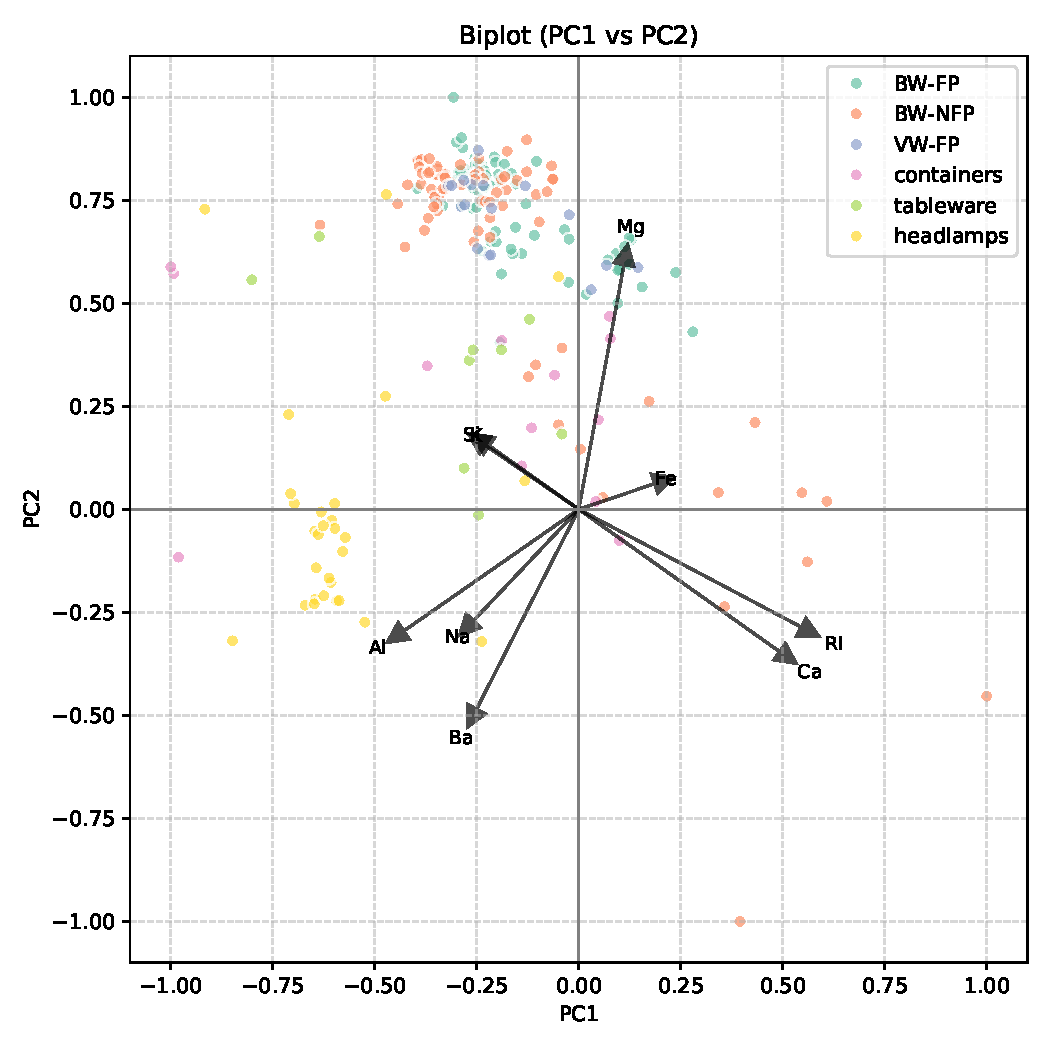
\includegraphics[width=\linewidth]{figures/pca_biplot_pc1_pc2.pdf}
			\caption{PC1 vs PC2}
			\label{fig:biplot_pc1_pc2}
		\end{subfigure}
		\hfill
		\begin{subfigure}{0.49\textwidth}
			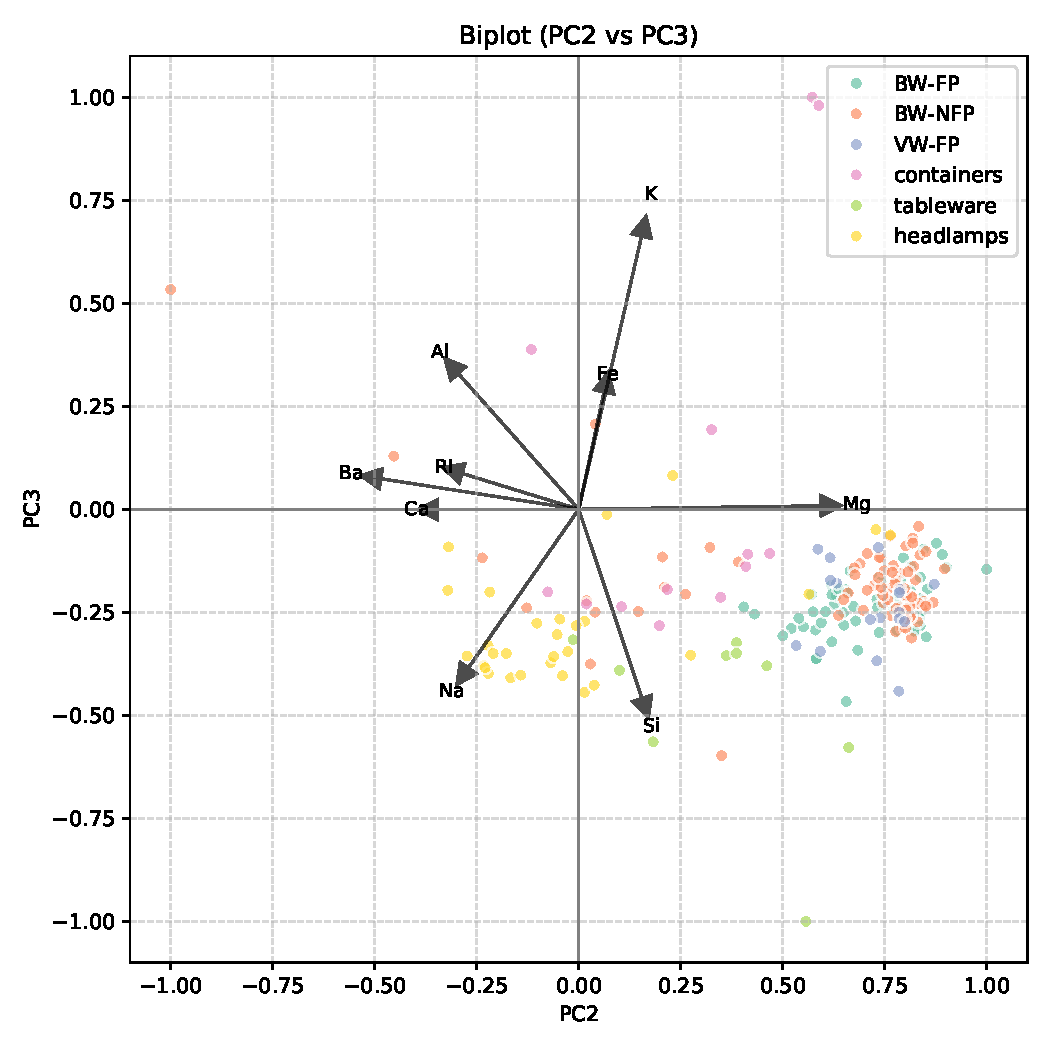
\includegraphics[width=\linewidth]{figures/pca_biplot_pc2_pc3.pdf}
			\caption{PC2 vs PC3}
			\label{fig:biplot_pc1_pc3}
		\end{subfigure}
		\caption{Biplots of the glass dataset showing both projected samples (colored by class) and variable loadings.}
		\label{fig:biplots}
	\end{figure}

	\subsubsection{Extreme scores}

	\todo{Explain the observations that score extremely high/low in certain principal directions.}

	\section{Use of GenAI}

	Keep in the back of your mind for what you used GenAI and add it at the end.

	\section*{Summary}

	\todo{Assignment: ``A discussion explaining what you have learned about the data.
		Summarize the most important things you have learned about the data and give your
		thoughts on whether your primary machine learning aim appears to be feasible based on
		your visualization.''}

	\bibliography{citations}
	\bibliographystyle{unsrt}

%	\newpage
%
%	\appendix
%
%	\LARGE\bfseries Appendix

%	\section{Test}

\end{document}